\begin{tikzpicture}
\begin{customlegend}[legend columns=2,legend style={align=left,draw=none,column sep=2ex}, legend cell align=left, %<= to align cells
legend entries={ % <= in the following there are the entries
Long stroke,
First short stroke,
Subsequent short stroke,
Enveloping curve,
Approximated first short stroke,
Approximated subsequent short stroke
}]
% legend style={at={(4.5,3.5)},font=\footnotesize}] % <= to define position and font legend
% the following are the "images" and numbers in the legend
    \addlegendimage{number in legend=1, black}
    \addlegendimage{number in legend=2, black}
    \addlegendimage{number in legend=3, black}
    \addlegendimage{number in legend=4, black}
    \addlegendimage{color=black!70, dotted, line width=3pt, line legend}
    \addlegendimage{color=black!40, dashed, line width=3pt}
\end{customlegend}
\end{tikzpicture}
\begin{tikzpicture}[scale=0.9]
\node[anchor=south west,inner sep=0] (image) at (0,0) {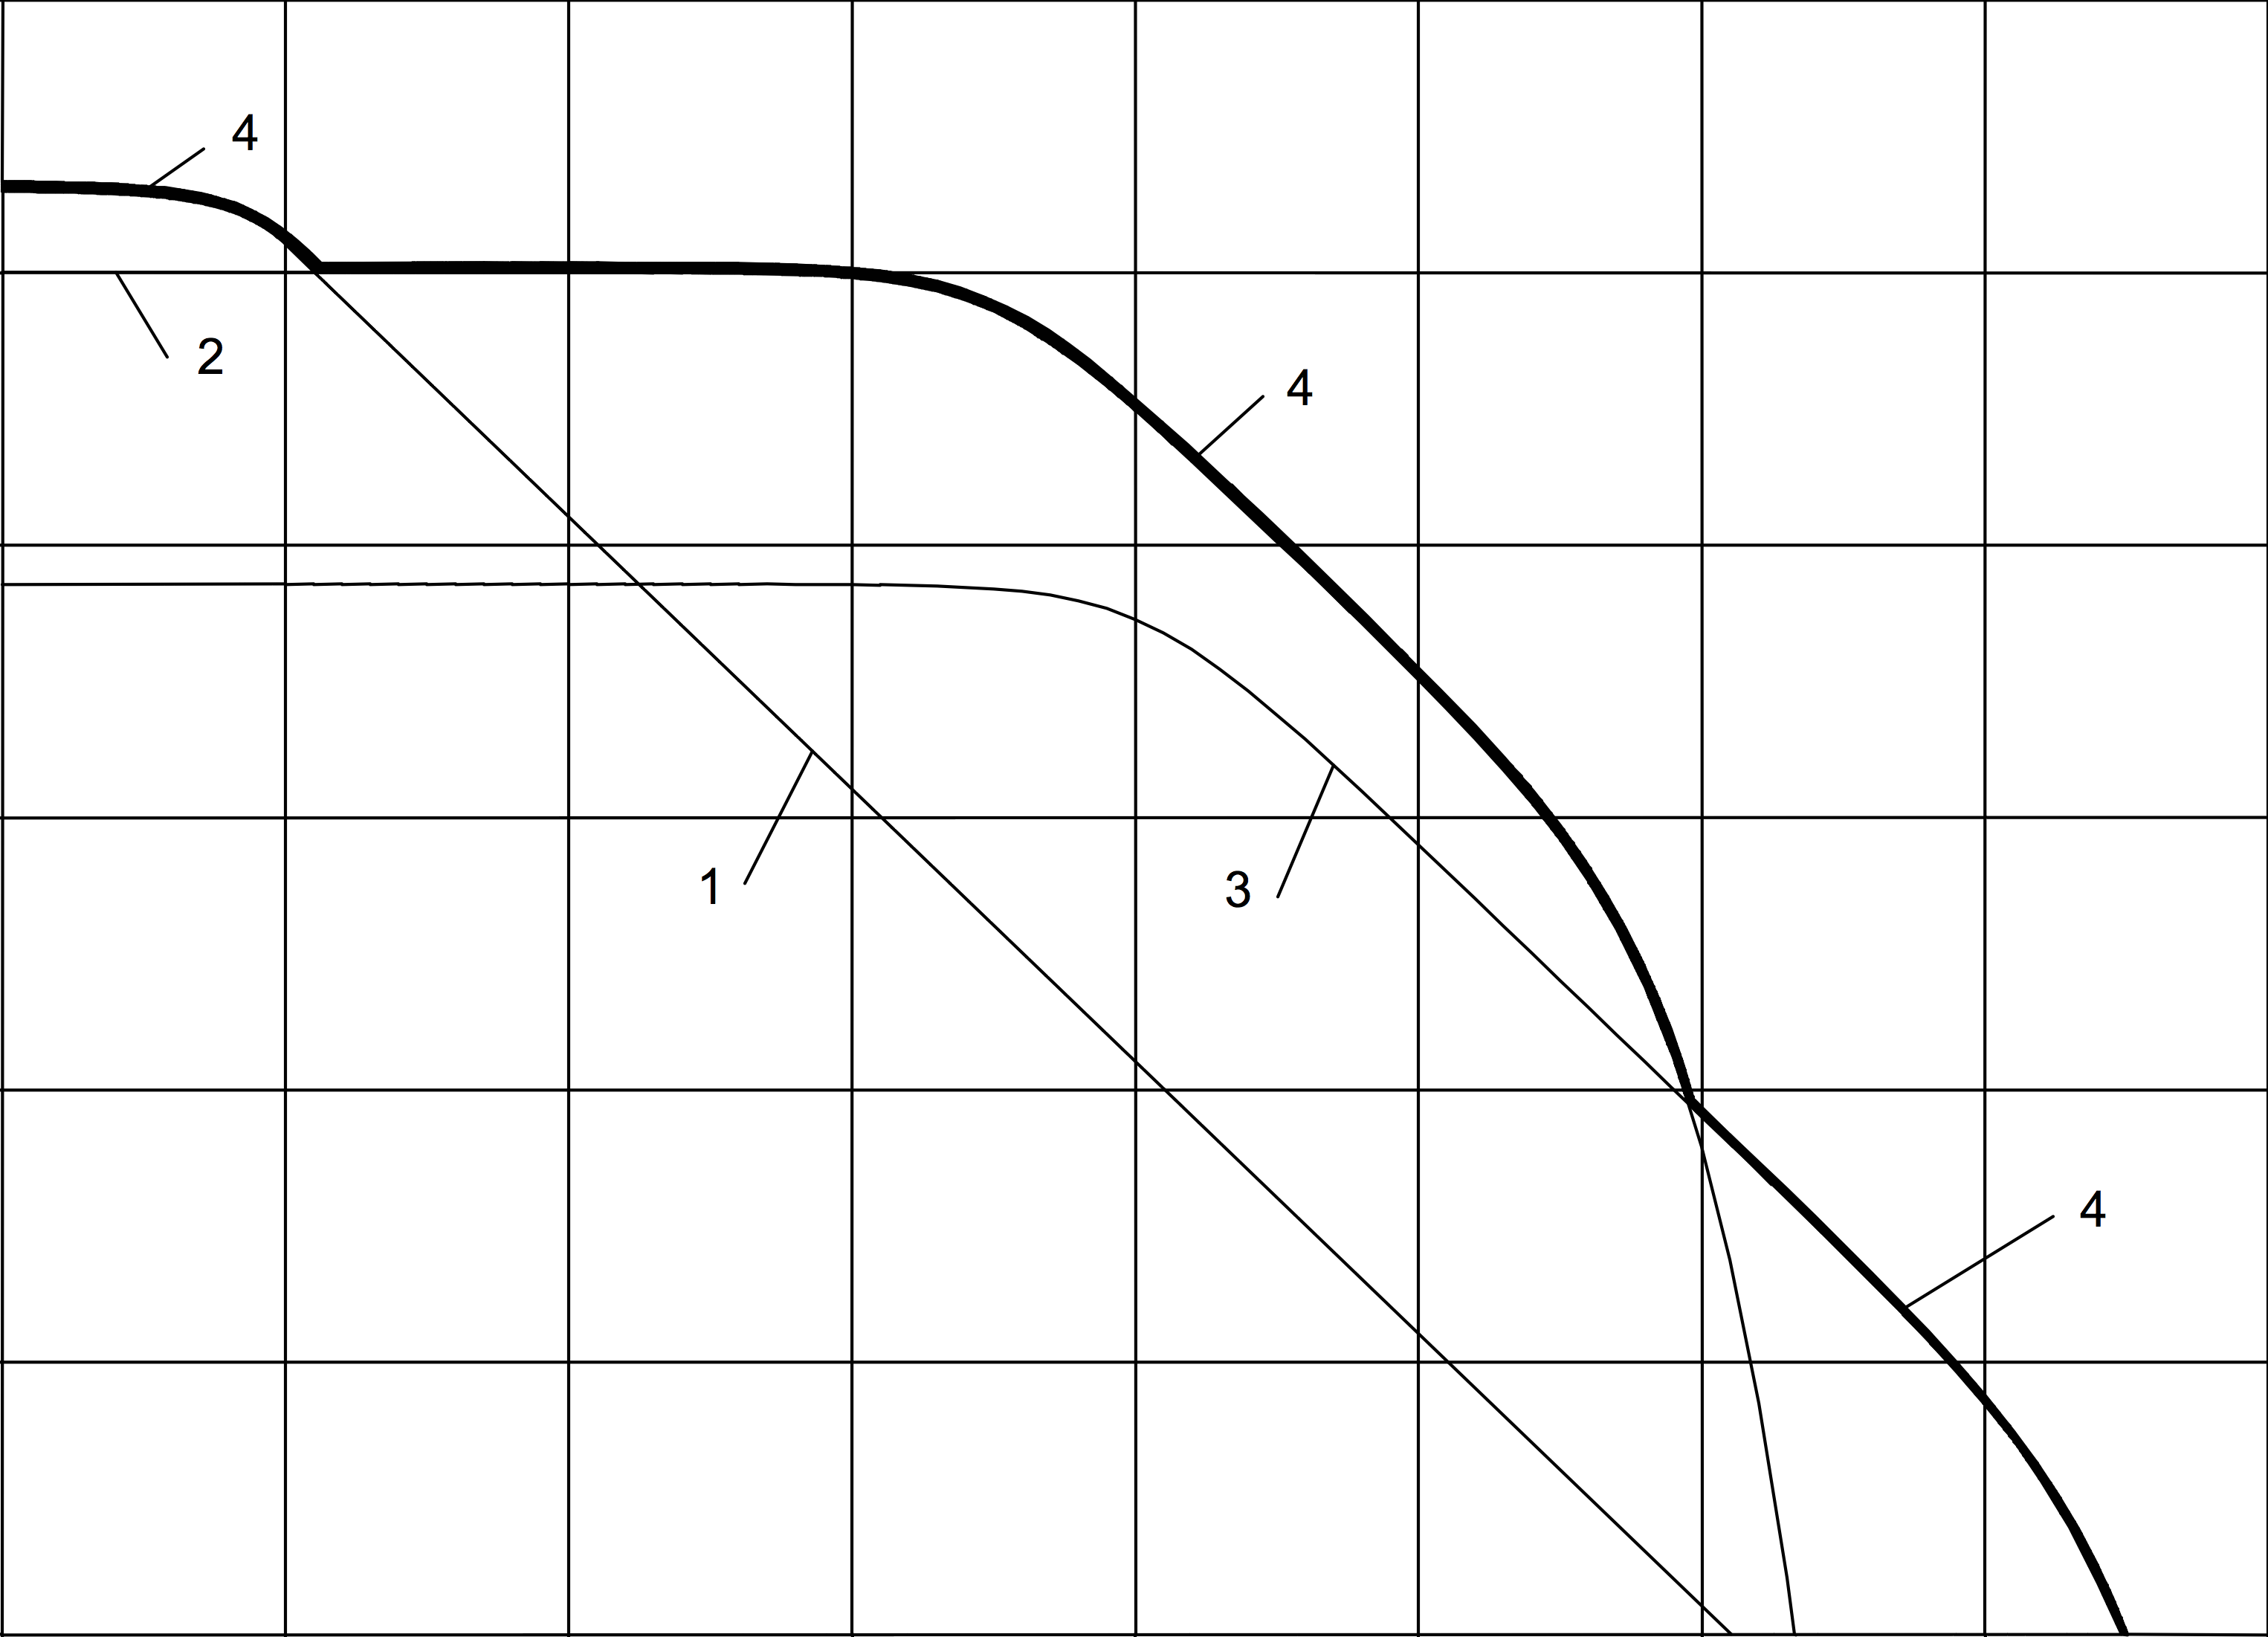
\includegraphics[width=0.72\linewidth, height=0.62\linewidth]{./Figures/Amplitude.png}};

\begin{axis}[%
width=0.8\linewidth,
scale only axis,
xmode=log,
xmin=0.1,
xmax=10000000,
% xminorticks=true,
% xmajorgrids,
ymode=log,
ymin=0.001,
ymax=1000,
% yminorticks=true,
% ymajorgrids,
ylabel={Current Density (A/Hz)},
xlabel={Frequency  (Hz)}
]

\addplot [color=black!70, dotted, line width=3pt]
  table[col sep=comma]{AdditionalFiles/FS/freqFS.csv};
% \addlegendentryexpanded{First Stroke};
\addplot [color=black!40, dashed, line width=3pt]
  table[col sep=comma]{AdditionalFiles/SS/freqSS.csv};
% \addlegendentryexpanded{Subsequent Stroke};
\end{axis}
\end{tikzpicture}%
